\documentclass[../thesis.tex]{subfiles}

\begin{document}
	
Trong thực tế một đối tượng luôn chịu tác động của nhiều yếu tố khác nhau. Để rút ra được bản chất của sự tương tác, sự ảnh hưởng, mức độ quan hệ của chúng, người ta phải xử lý số liệu nhiều chiều. Cùng với sự phát triển của thống thống kê nhiều chiều, sự phát triển của công nghệ thông tin đã giúp chúng ta xử lý khá hiệu quả số liệu nhiều chiều. 

\section{Dẫn nhập}
Phân tích thành phần chính (principle component analysis, PCA) là phương pháp dựa trên việc tối đa lượng thông tin
được giữ lại. Nó đi tìm một phép xoay trục toạ độ để được một hệ trục toạ độ\index{trục toạ độ} mới sao cho trong hệ mới này, thông tin của dữ liệu chủ yếu tập trung ở một vài thành phần. Phần còn lại chứa ít thông tin hơn có thể được lược bỏ.

\begin{SCfigure}
	\centering
	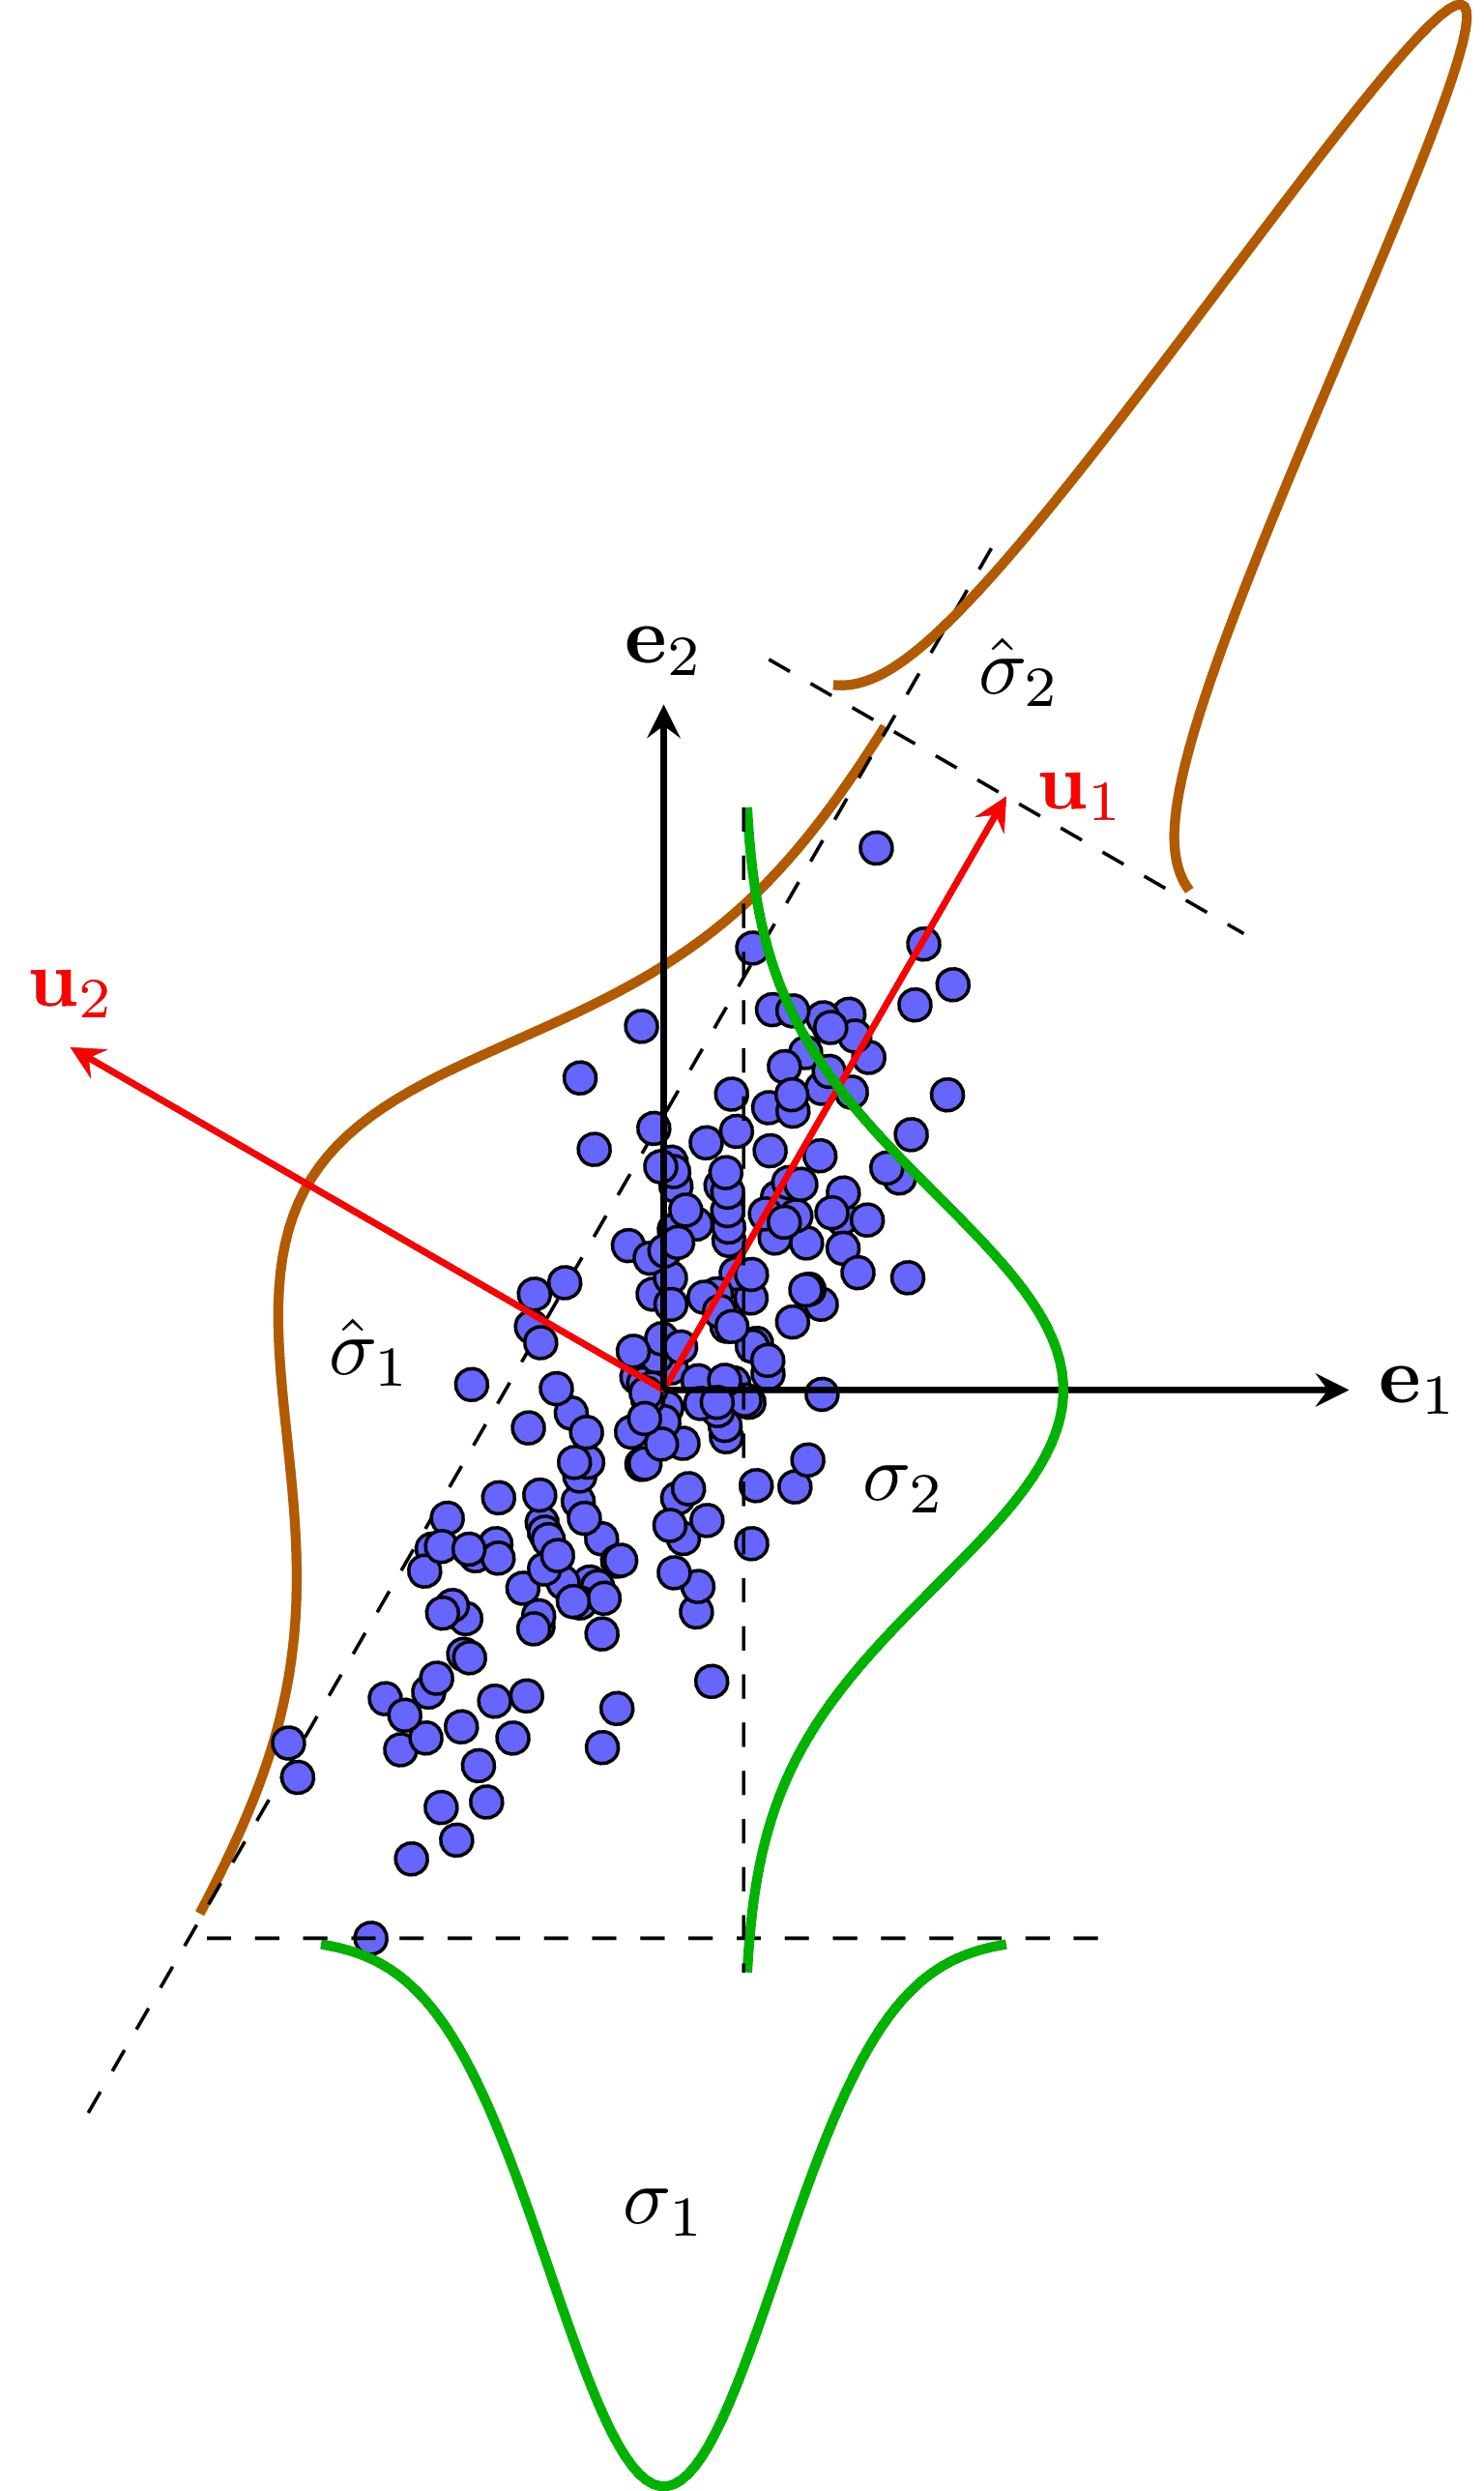
\includegraphics[width=0.5\linewidth]{images/pca_var}
	\caption[Mô tả thuật toán phân tích thành phần chính]{\protect Phân tích thành phần chính có thể được coi là phương pháp đi tìm một hệ cơ sở trực chuẩn đóng vai trò một phép xoay, sao cho trong hệ cơ sở mới này, phương sai theo một số chiều nào đó là không đáng kể và có thể lược bỏ. Trong hệ cơ sở ban đầu $ \mathbf{O}\mathbf{e}_1\mathbf{e}_2 $, phương sai theo mỗi chiều (độ rộng của các đường hình chuông màu xanh lá) đều lớn. Trong không gian mới với hệ cơ sở $ \mathbf{O}\mathbf{u}_1\mathbf{u}_2 $, phương sai theo hai chiều (độ rộng của các đường hình chuông) chênh lệch nhau đáng kể. Chiều dữ liệu có phương sai nhỏ có thể được lược bỏ vì dữ liệu theo chiều này ít phân tán. Nguồn: Machine Learning cơ bản \cite{VuHuuTiep}}
	\label{fig:pcavar}
\end{SCfigure}

Hình~\ref{fig:pcavar} minh hoạ các thành phần chính với dữ liệu hai chiều.
Trong không gian ban đầu với các vector cơ sở $\mathbf{e}_1\,,\mathbf{e}_2$, phương sai theo mỗi chiều dữ liệu (tỉ lệ với độ rộng của các hình chuông màu nâu) đều lớn. Trong hệ cơ sở mới $\mathbf{O}\mathbf{u}_1\mathbf{u}_2$, phương sai theo chiều thứ hai $\hat{\sigma}_2^2$ nhỏ so với $\hat{\sigma}_1^2$. Điều này chỉ ra rằng khi chiếu dữ liệu lên $\mathbf{u}_2$, ta được các điểm rất gần nhau và gần với giá trị trung bình theo chiều đó. Trong trường hợp này, vì giá trị trung bình theo mọi chiều bằng 0, ta có thể thay thế toạ độ theo chiều $\mathbf{u}_2$ bằng 0. Rõ ràng là nếu dữ liệu có phương sai càng nhỏ theo một chiều nào đó thì khi xấp xỉ chiều đó bằng một hằng số, sai số xấp xỉ càng nhỏ. PCA thực chất là đi tìm một phép xoay tương ứng với một ma trận trực giao sao cho trong hệ toạ độ mới, tồn tại các chiều có phương sai nhỏ có thể được bỏ qua; ta chỉ cần giữ lại các chiều/thành phần khác quan trọng hơn. Như đã khẳng định ở trên, tổng phương sai theo toàn bộ các chiều trong một hệ cơ sở bất kỳ là như nhau và bằng tổng các trị riêng của ma trận hiệp phương sai. Vì vậy, PCA còn được coi là phương pháp giảm số chiều dữ liệu sao cho tổng phương sai còn lại là lớn nhất. \cite{VuHuuTiep}. 

\section{Thuật toán phân tích thành phần chính}

Phân tích thành phần chính là kĩ thuật biểu diễn số liệu dựa theo các tiêu chuẩn về đại số và hình học mà không đòi hỏi một giả thuyết thống kê hay mô hình đặc biệt nào. Mục đích của phân tích thành phần chính là rút ra thông tin chủ yếu chứa trong  bảng số liệu bằng cách xây dựng một biểu diễn đơn giản hơn sao cho đám mây số  liệu được thể hiện rõ nhất. Cụ thể hơn, phân tích thành phần chính tức là đi tìm  những trục hay mặt phẳng "phản ánh" tốt nhất, trung thực nhất đám mây điểm - biến, điểm - cá thể. 

Với bảng số liệu có rất nhiều cột dòng, mỗi cột là một biến, mỗi dòng là một cá  thể, trên đó đo đồng thời giá trị các biến, giữa các cá thể qua thể hiện rõ nhất trong  một không gian con số chiều ít hơn.

Từ các suy luận trên, ta có thể tóm tắt lại các bước trong PCA như sau: 
\begin{itemize}
	\item[1)] Tính véc-tơ trung bình của toàn bộ dữ liệu:
	\begin{math} 
		\bar{\mathbf{x}} = \frac{1}{n} \sum_{n=1}^n \mathbf{x}_n 
	\end{math}.
	\item[2)] Trừ mỗi điểm dữ liệu đi véc-tơ trung bình của toàn bộ dữ liệu để được dữ
	liệu chuẩn hoá:
	\begin{equation*} 
		\hat{\mathbf{x}}_n = \mathbf{x}_n - \bar{\mathbf{x}} 
	\end{equation*} 
	\item[3)] Đặt $\widehat{\mathbf{X}} = [\widehat{\mathbf{x}}_1, \widehat{\mathbf{x}}_2, \dots,
	\widehat{\mathbf{x}}_d]$ là ma trận dữ liệu chuẩn hoá, tính ma trận hiệp phương sai: $$ \mathbf{S} = \frac{1}{n}\widehat{\mathbf{X}}\widehat{\mathbf{X}}^\top $$
	\item[4)] Tính các trị riêng và véc-tơ riêng tương ứng có $\ell_2$ chuẩn bằng 1
	của ma trận này, sắp xếp chúng theo thứ tự giảm dần của trị riêng.
	\item[5)] Chọn $K$ véc-tơ riêng ứng với $K$ giá trị riêng lớn nhất để xây dựng ma trận $\mathbf{U}_K$ có các cột tạo thành một hệ trực giao. $K$ vector này được gọi là các thành phần chính, tạo thành một không gian con (gần) với phân bố của dữ liệu ban đầu đã chuẩn hoá. 
	\item[6)] Chiếu dữ liệu ban đầu đã chuẩn hoá $\widehat{\mathbf{x}}$ xuống không gian con tìm được. 
	\item[7)] Dữ liệu mới là toạ độ của các điểm dữ liệu trên không gian mới: $$ \mathbf{Z} = \mathbf{U}_K^\top\widehat{\mathbf{X}}$$
\end{itemize}

Như vậy, thuật toán phân tích thành phần chính là thuật toán kết hợp của phép tịnh tiến, xoay trục toạ độ và chiếu dữ liệu lên hệ toạ độ mới.

\begin{figure}[H]
	\centering
	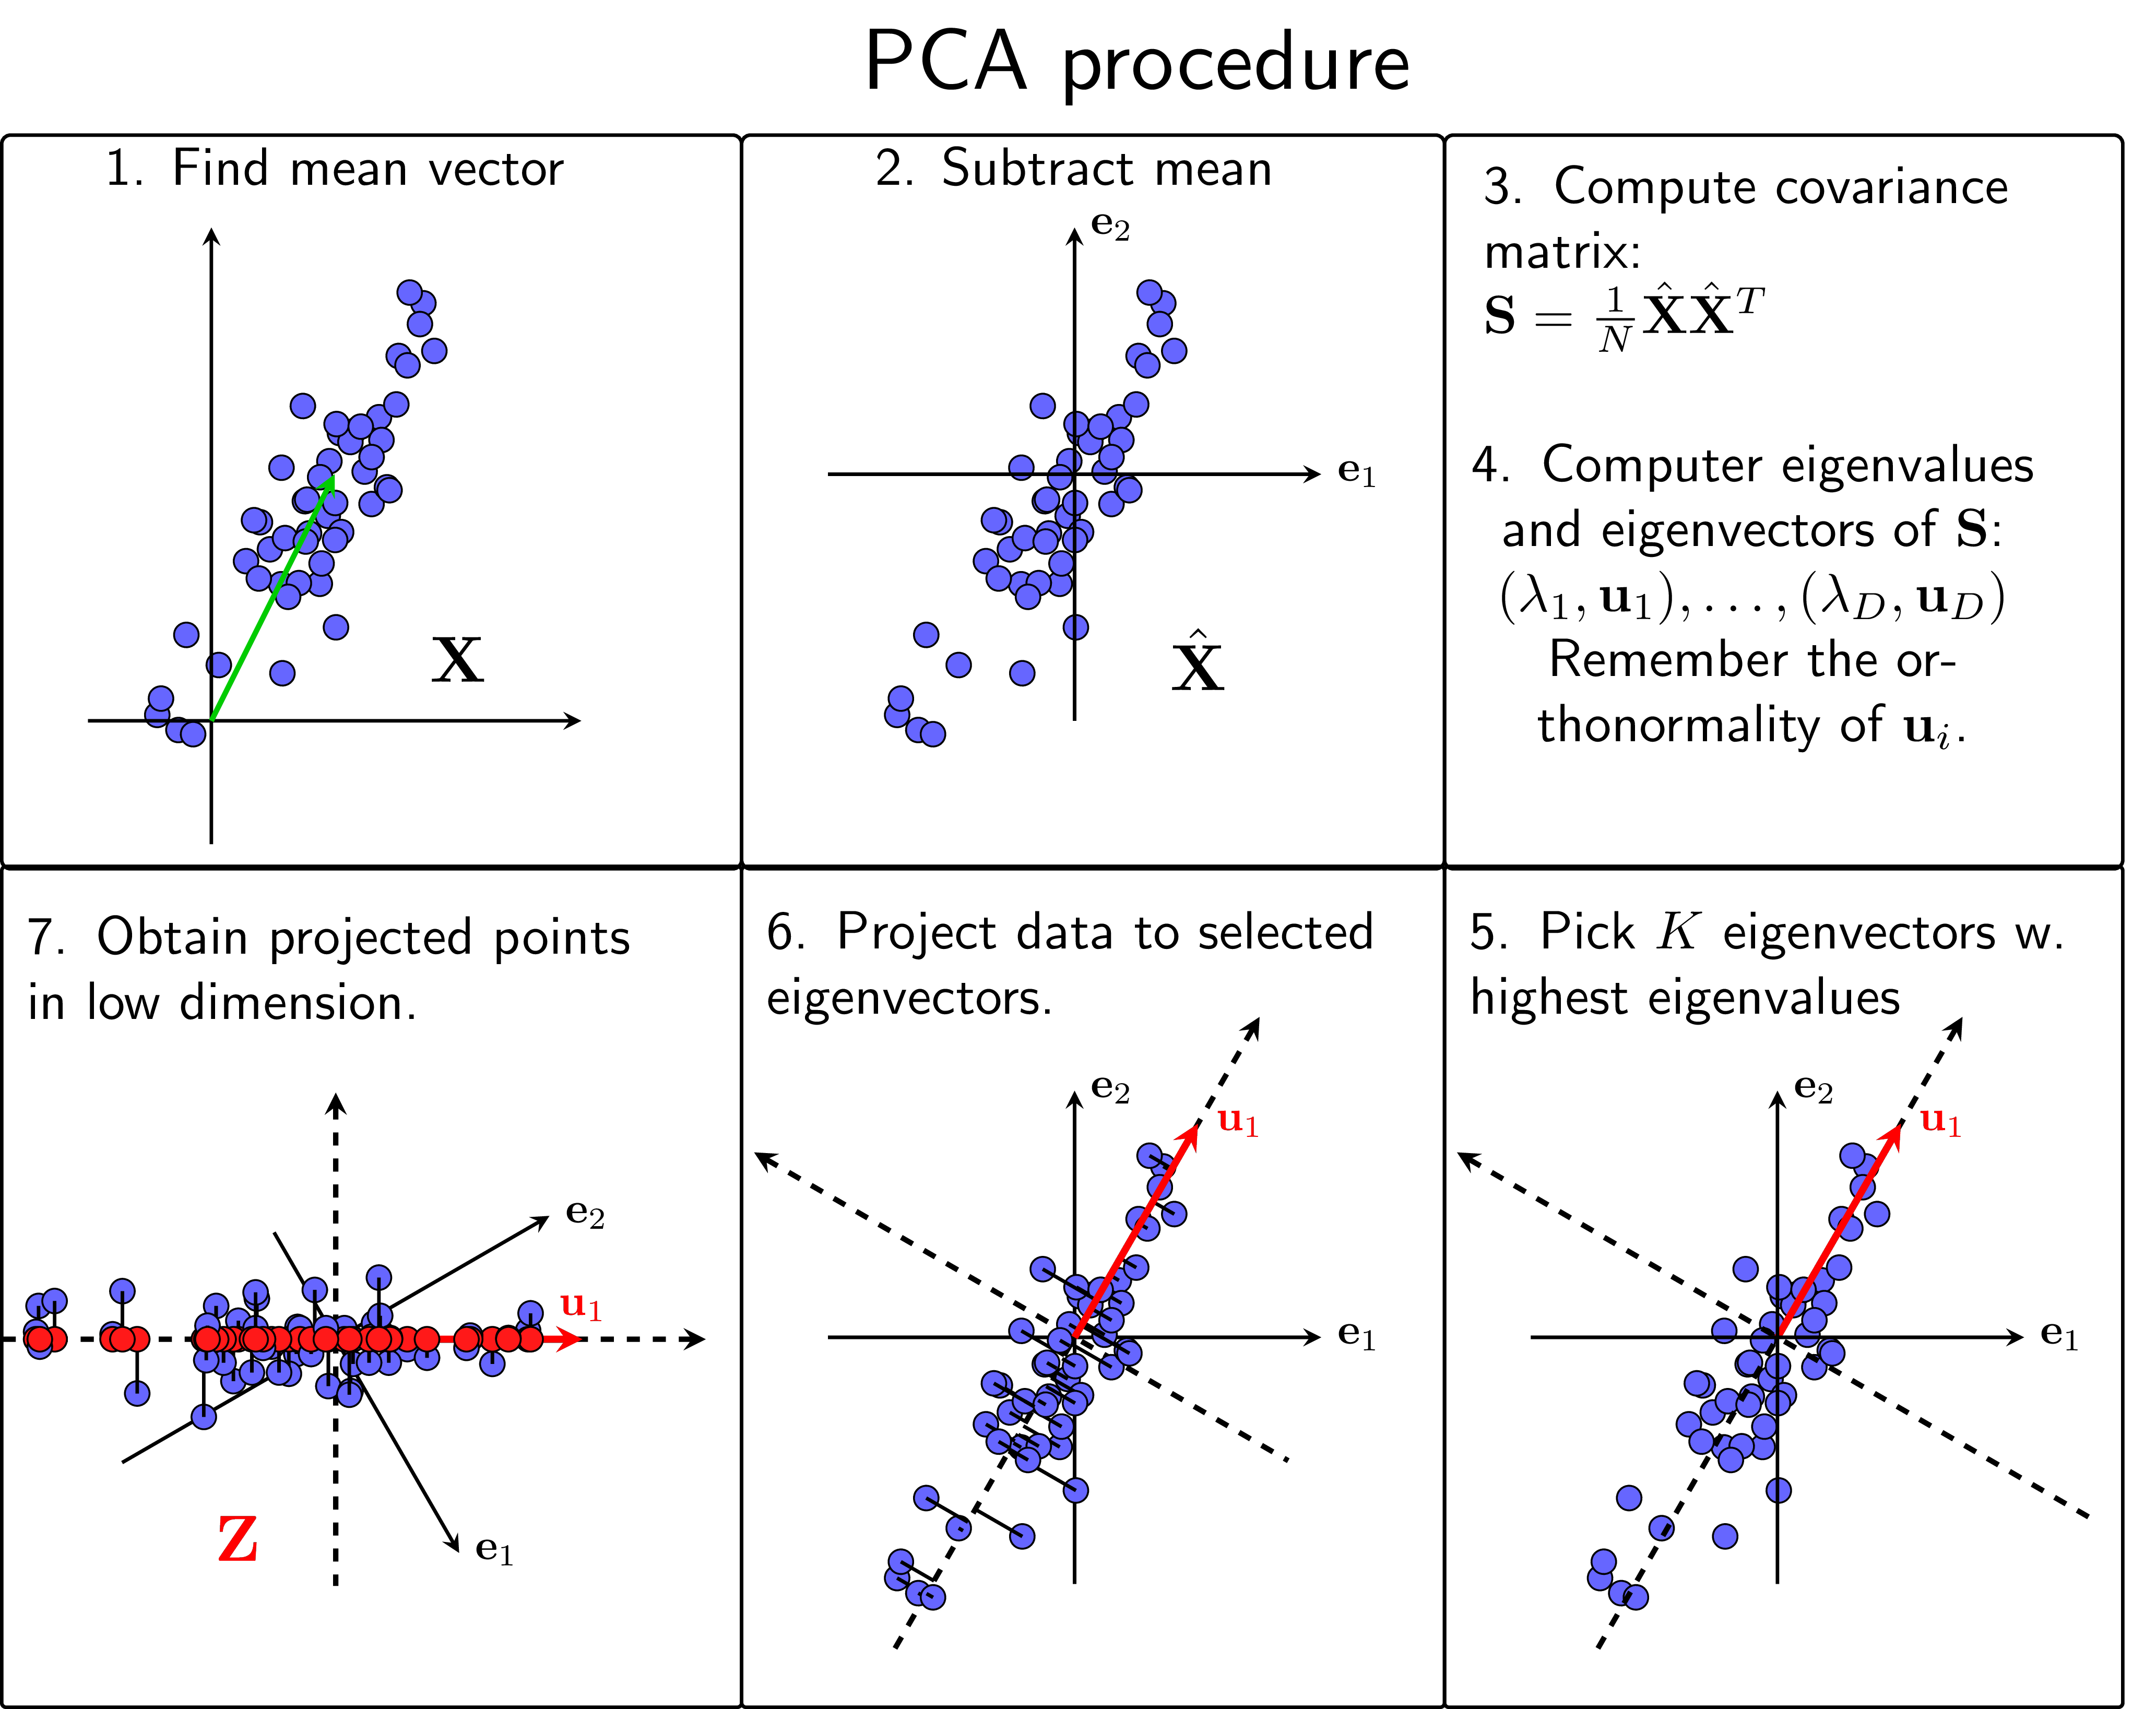
\includegraphics[width=0.8\linewidth]{images/pca_procedure}
	\caption[Thuật toán phân tích thành phần chính]{Thuật toán phân tích thành phần chính. Bước 1. Tìm véc-tơ trung bình; Bước 2. Lấy dữ liệu trừ lần lượt cho véc-tơ trung bình; Bước 3. Tính ma trận hiệp phương sai $ \mathbf{S} = \frac{1}{n}\widehat{\mathbf{X}} \widehat{\mathbf{X}}^\top $; Bước 4. Tìm giá trị riêng và véc-tơ riêng của ma trận hiệp phương sai $ \mathbf{S} $ lần lượt là $ (\lambda_1\,,\mathbf{u}_1)\,,\ldots\,,(\lambda_D\,,\mathbf{u}_D) $, các véc-tơ riêng được chọn phải tạo thành một hệ trực chuẩn; Bước 5. Chọn $ K $ véc-tơ riêng ứng với giá trị riêng lớn nhất; Bước 6. Chiếu dữ liệu ban đầu xuống các véc-tơ riêng đó; Bước 7. Dữ liệu giảm chiều (các điểm màu đỏ)}
	\label{fig:pcaprocedure}
\end{figure}

\section{Tiêu chí giảm thiểu số chiều dữ liệu}
Phân tích thành phần chính (viết tắt là PCA) là một cách tiếp cận đa biến nổi tiếng chuyển đổi một số biến tương quan thành một số biến không tương quan tuyến tính được đặt tên là các thành phần chính. Trong chuyển đổi này, các thành phần chính đầu tiên chứa nhiều thông tin nhất về tập dữ liệu. Trong các ứng dụng, PCA được áp dụng để chuyển đổi tập dữ liệu chiều cao thành tập dữ liệu chiều thấp hơn, bằng cách chỉ sử dụng một số thành phần chính đầu tiên để giảm kích thước của dữ liệu được biến đổi. Dựa trên Chỉ số Kaiser\index{chỉ số Kaiser}, số lượng các thành phần chính quan trọng bằng số lượng các giá trị riêng của ma trận tương quan với các giá trị lớn hơn 1.

\begin{enumerate}
	\item Lựa chọn những thành phần chính để giải thích một tỷ lệ nhất định (ví dụ $ 95\% $) của $ trace(\bm{\Lambda}) $. Đây là một tiêu chí đơn giản nhưng không được khuyến cáo.
	\item Hầu hết, cách tiếp cận để xác định số lượng thành phần chính bằng cách xác định giá trị riêng thông qua ma trận hệ số tương quan giữa dần đến khi số lượng thành phần chính bằng số biến). Kaiser -- Harris đề xuất, thành phần chính được xác định khi giá trị riêng có giá trị lớn hơn 1.
	\item Tiêu chuẩn Guttma -- Kaise\index{tiêu chuẩn Guttma -- Kaise} loại bỏ các giá trị riêng dưới mức trung bình $ \tfrac{trace(\bm{\Lambda})}{d} $ (dưới 1 đối với dữ liệu chuẩn hóa), điều này có nghĩa là giảm các thành phần có phương sai được đóng góp bởi một biến nếu biến tổng được phân phối đều nhau
\end{enumerate}

\newpage
\section*{Tổng kết chương}

Trong chương thuật toán phân tích thành phần chính này ta sẽ nói về 4 thành phần chính

Đầu tiên là dẫn nhập, ta sẽ tìm hiểu rõ phân tích thành phần chính là gì và chức năng của nó như thế nào. Phân tích thành phần chính có tên tiếng Anh là (principle component analysis, PCA) là phương pháp dựa trên việc tối đa
lượng thông tin được giữ lại. Chức năng của nó là đi tìm một phép xoay trục toạ độ để được một hệ trục toạ độ mới sao cho trong hệ mới này, thông tin của dữ liệu chủ yếu tập trung ở một vài thành phần. 

Thứ hai là thuật toán phân tích thành phần chính, ta sẽ đi sâu vào mục đích của phân tích thành phần chính, đặc biệt là với bảng số liệu sẽ như thế nào. Mục đích của phân tích thành phần chính là rút ra thông tin chủ yếu chứa trong bảng số liệu bằng cách xây dựng một biểu diễn đơn giản hơn sao cho đám mây số liệu được thể hiện rõ nhất. Còn với bảng số liệu có rất nhiều cột dòng, mỗi cột là một biến, mỗi dòng là một cá thể, trên đó đo đồng thời giá trị các biến, giữa các cá thể qua thể hiện rõ nhất trong một không gian con số chiều ít hơn.

Thứ ba là tiêu chí giảm thiểu số chiều dữ liệu. Ở đây ta sẽ có 2 tiêu chí là 1) Lựa chọn những thành phần chính để giải thích một tỷ lệ nhất định (ví dụ $ 95\% $) của $ trace(\bm{\Lambda}) $; 2)  Tiêu chuẩn Guttma – Kaise loại bỏ các giá trị riêng dưới mức trung bình $ trace(\bm{\Lambda}) $.

\end{document}
